Energy price prediction is a cumbersome task to handle because of the highly volatile nature of such predictions \cite{pjmForecast, yamin2004adaptive} and the plethora of factors that influence the energy price\cite{singhal2011electricity}. In this section we will show the factors that influence the price by analyzing relevant data that will later become input in our ANN. Not too surprisingly; the most important factor in any market is \fnurl{demand}{http://en.wikipedia.org/wiki/Supply_and_demand} and this greatly influences the price. Time of day, day of the week, wind speed and temperature (that are the quantifiable factors) also play a big role. Sociocultural influences affects the price as well but are hard to measure \cite{singhal2011electricity}. This section will show the connection between electricity price and the influential factors.

\noindent The price throughout this thesis is represented in DKK the danish currency.

\subsection{Price}\label{sec:Price}
We present some of the influences on the price in this section and argue why these parameters have an impact on the price. We also account for the time perspective and show the non-linear nature of energy prices. To accompany the graphs we also calculated the Pearson's correlations (Section ~\ref{sec:Pearsons}) that can be seen in Table~\ref{table:pearsonsPriceVariables}.

Pearson's correlations:
\begin{table}[H]
\centering  % used for centering table
\begin{tabular}{|c|c|c|} % centered columns
 \hline
 Parameter 1 & Parameter 2 & Pearsons \\ [0.5ex] % inserts table 
%heading
\hline                  % inserts single horizontal line
Price & Demand & 0.31 \\ \hline
Price & Wind speed & -0.28  \\ \hline
Price & Temperature & -0.18 \\ \hline
Price & Last known price & 0.89 \\ \hline
Demand & Wind speed & 0.57 \\ \hline
Demand & Temperature & -0.59 \\ \hline
\end{tabular}
\caption{Pearson's correlations for price prediction variables} % title of Table
\label{table:pearsonsPriceVariables} % is used to refer this table in the text
\end{table}

The last known price has a great correlation to the price we are going to predict that can be seen in Figure~\ref{fig:price_price} and by the Pearsons correlation of 0.89. Even though the price is volatile and have spikes it follows a pattern; that clearly shows us that the historical price development is very important when predicting the next prices.

\begin{figure}[H]
\centering
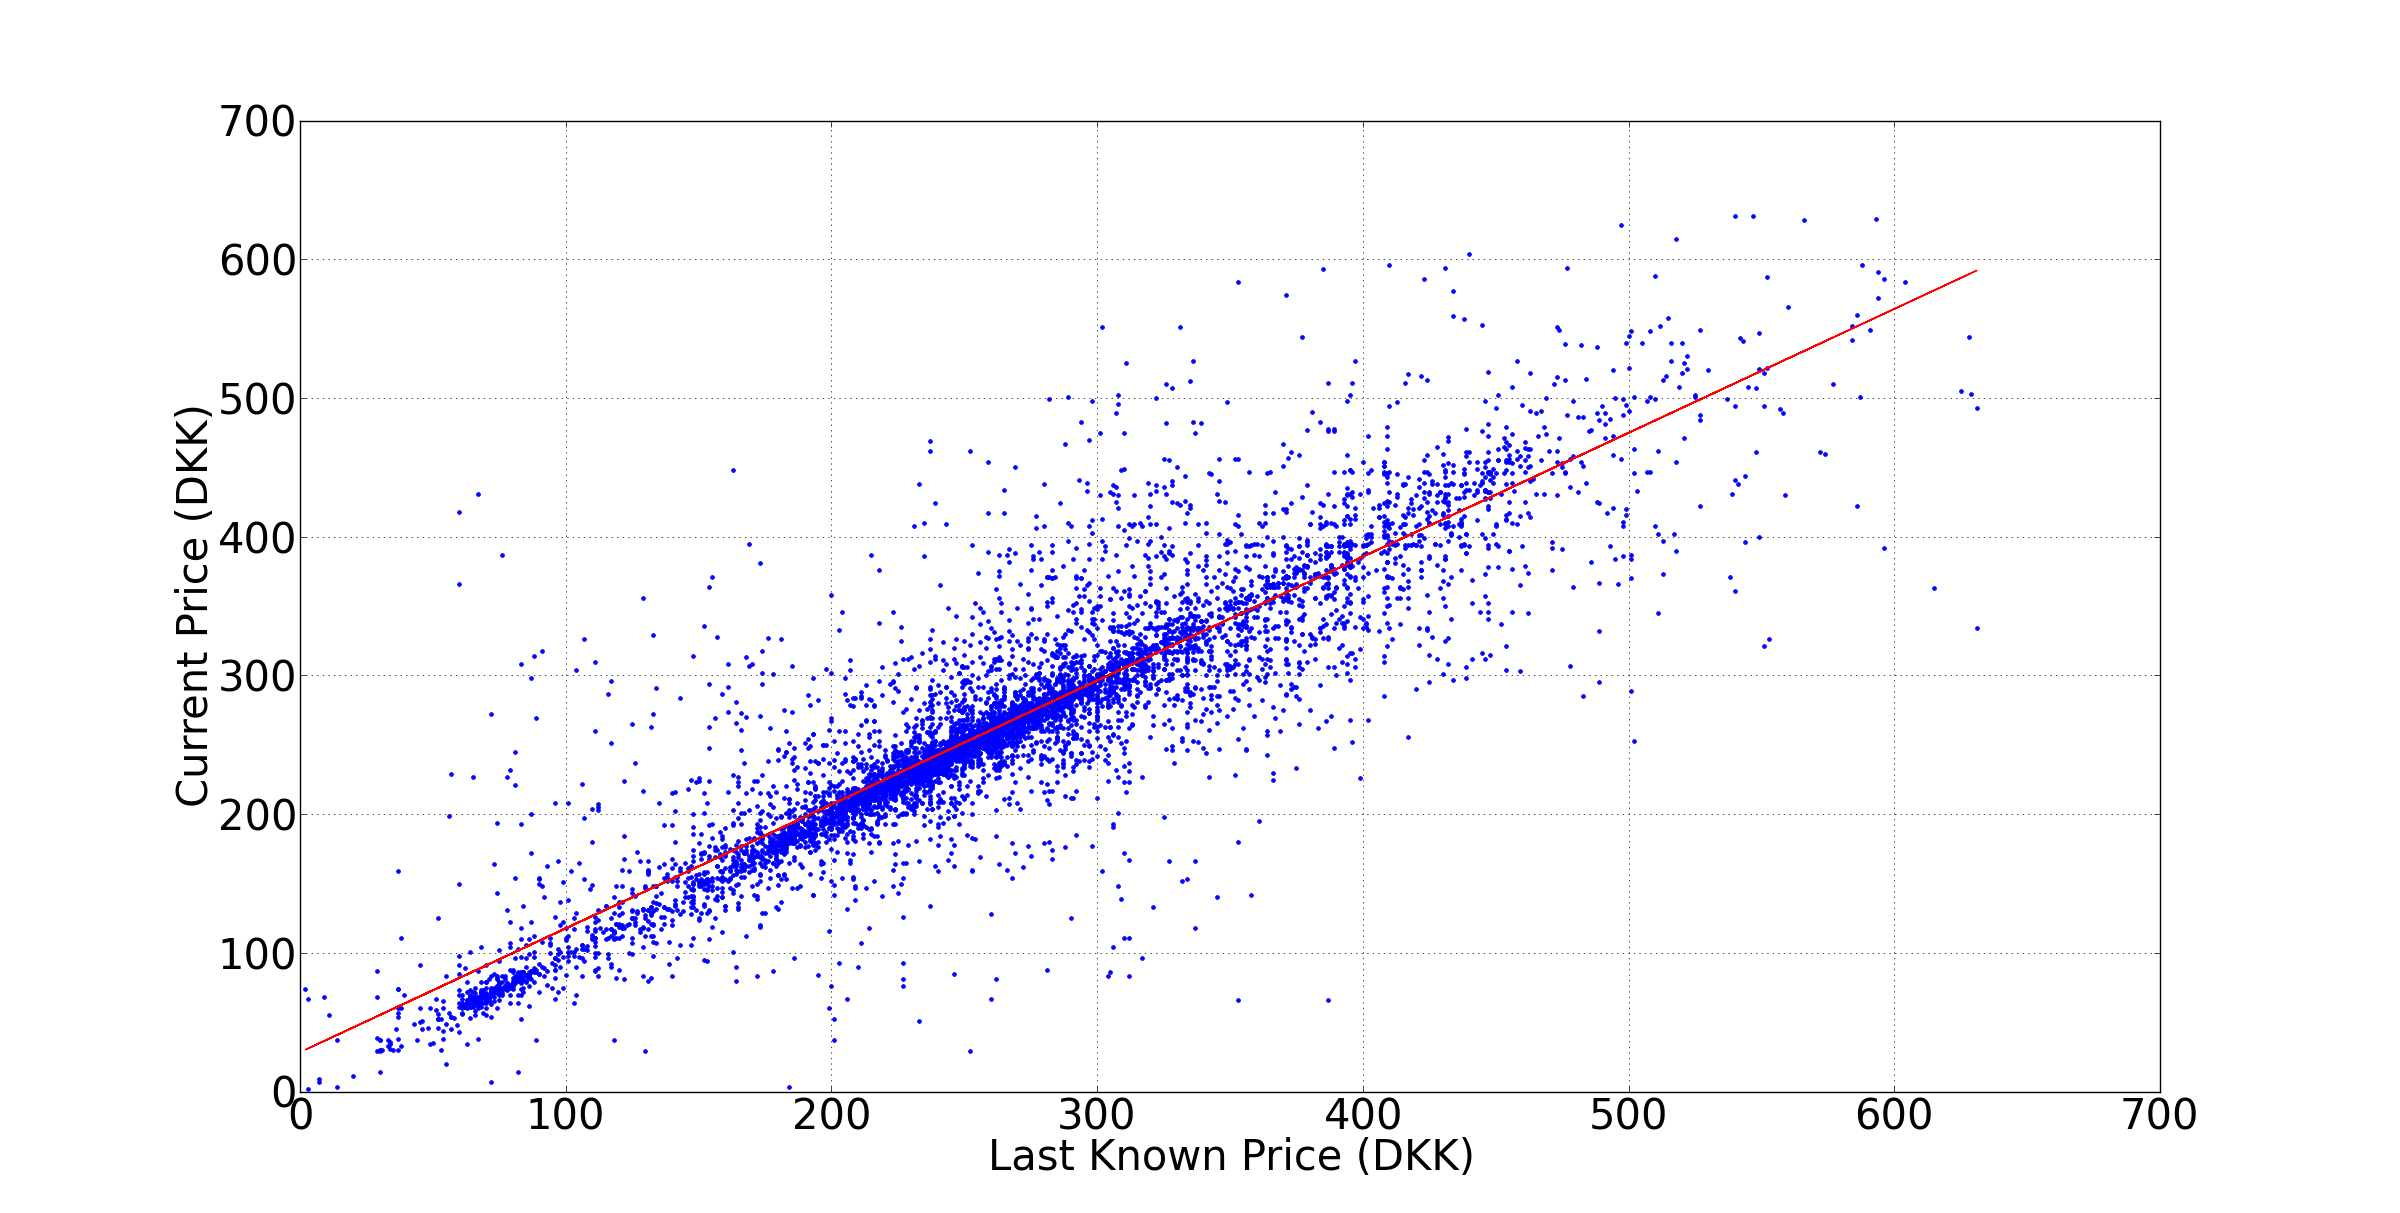
\includegraphics[width=0.99\textwidth]{billeder/priceVsLastKnownPrice.png}
\caption{Price and last known price}
\label{fig:price_price}
\end{figure}

The correlation between the last known price and the price to be predicted shows how important the movement of the curve is when predicting the price can also be seen in Figure \ref{fig:priceGraphFirst400Hours}. Therefore further analysis about curve movement might help the ANN to better predictions if we can foresee the most likely way for the graph to move e.g. if the price is close to the max price it might soon start to drop again 

\begin{figure}[H]
\centering
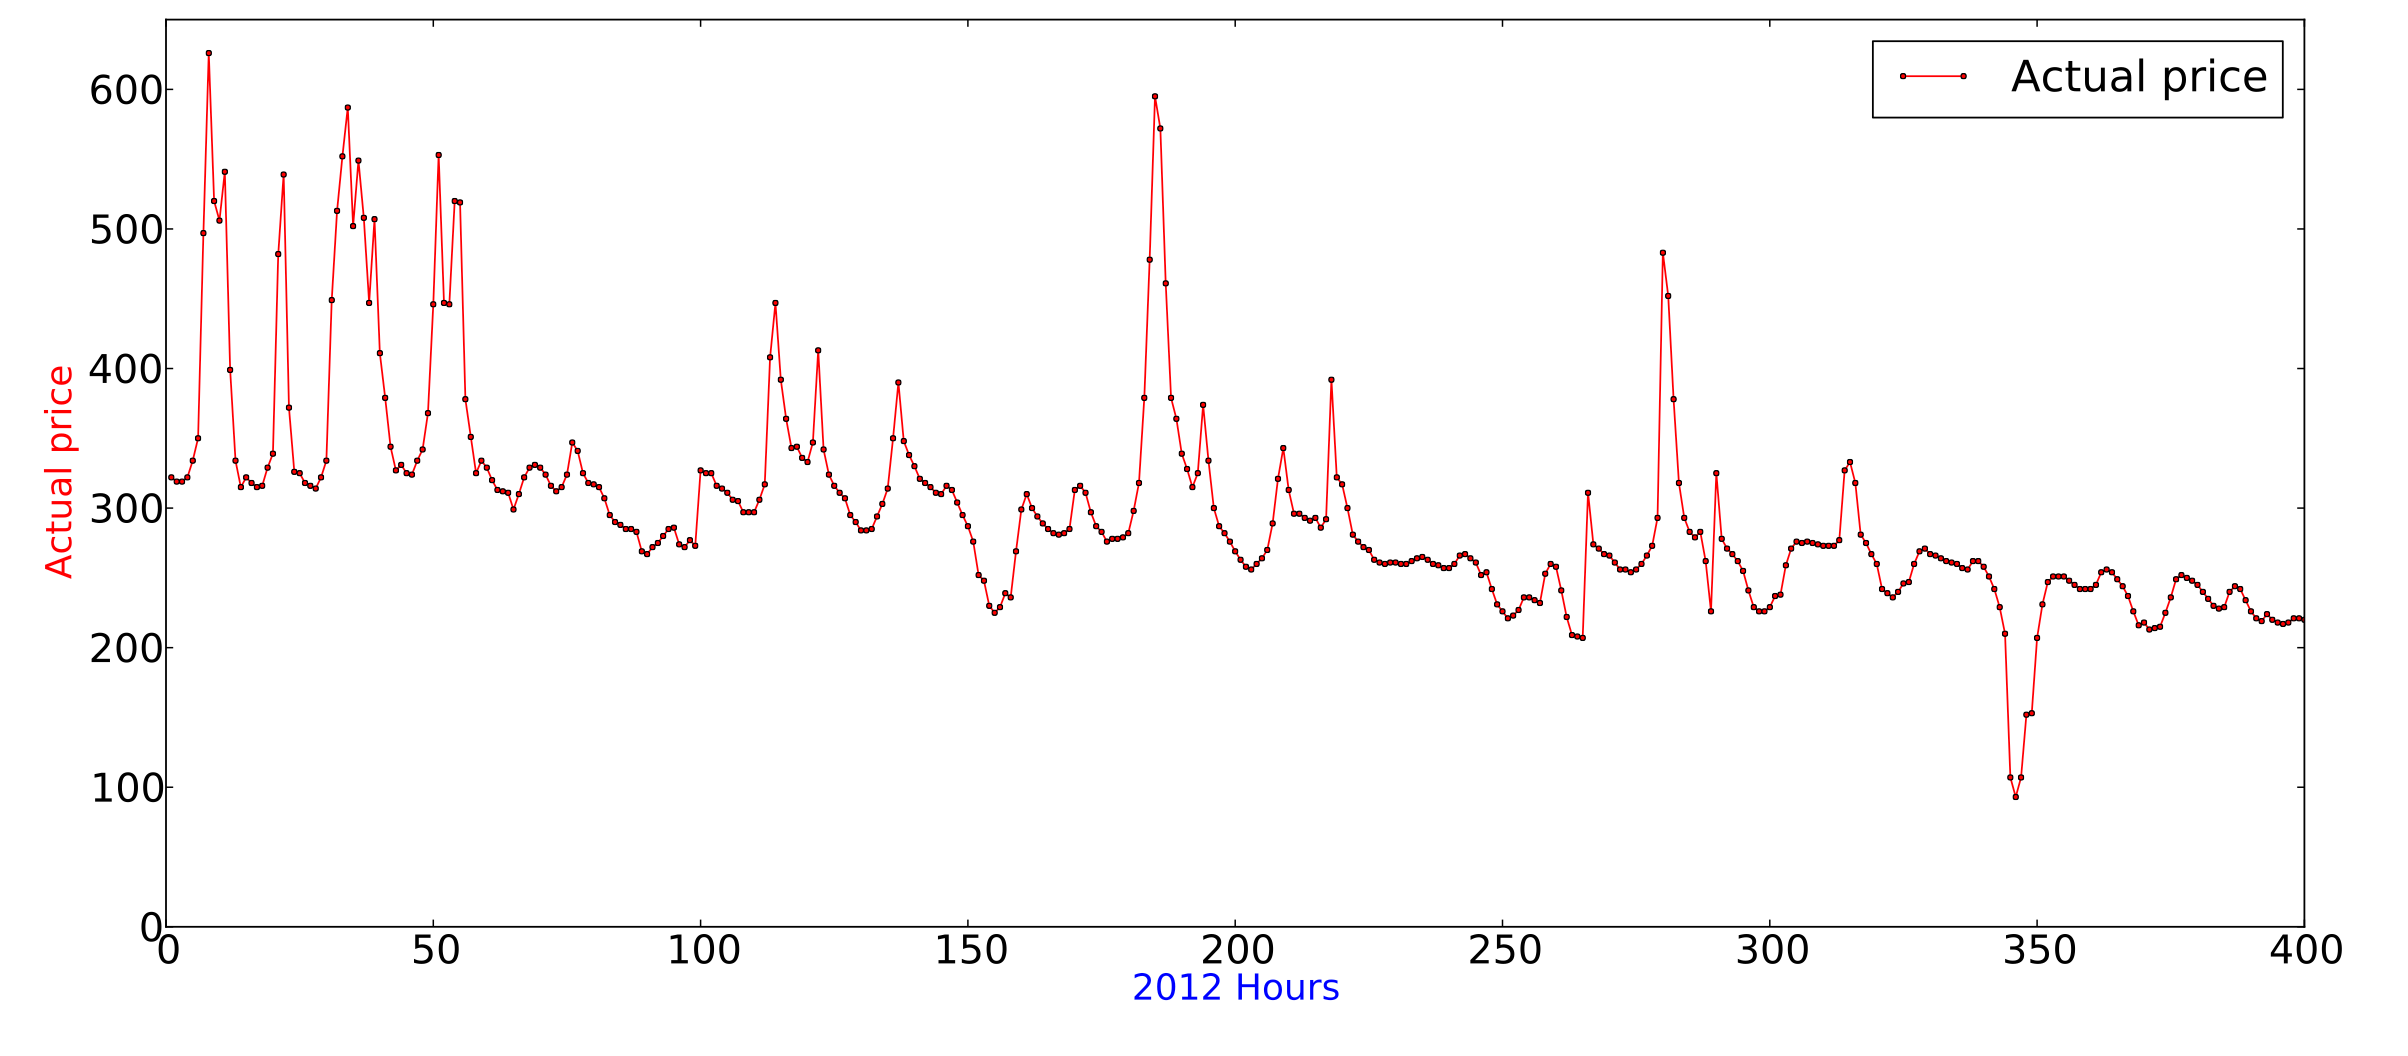
\includegraphics[width=0.99\textwidth]{billeder/priceGraph400.png}
\caption{The price movement in the first 400 hours of 2012.}
\label{fig:priceGraphFirst400Hours}
\end{figure}

%------------------------------------------------------------------------------------------------------------------------------
\subsubsection{Weather conditional influences}
\label{sec:priceWeatherInfluence}
The electricity price is affected by different weather conditions. We present temperature and wind speed and show how the correlation between them and the price is.

\begin{figure}[H]
\centering
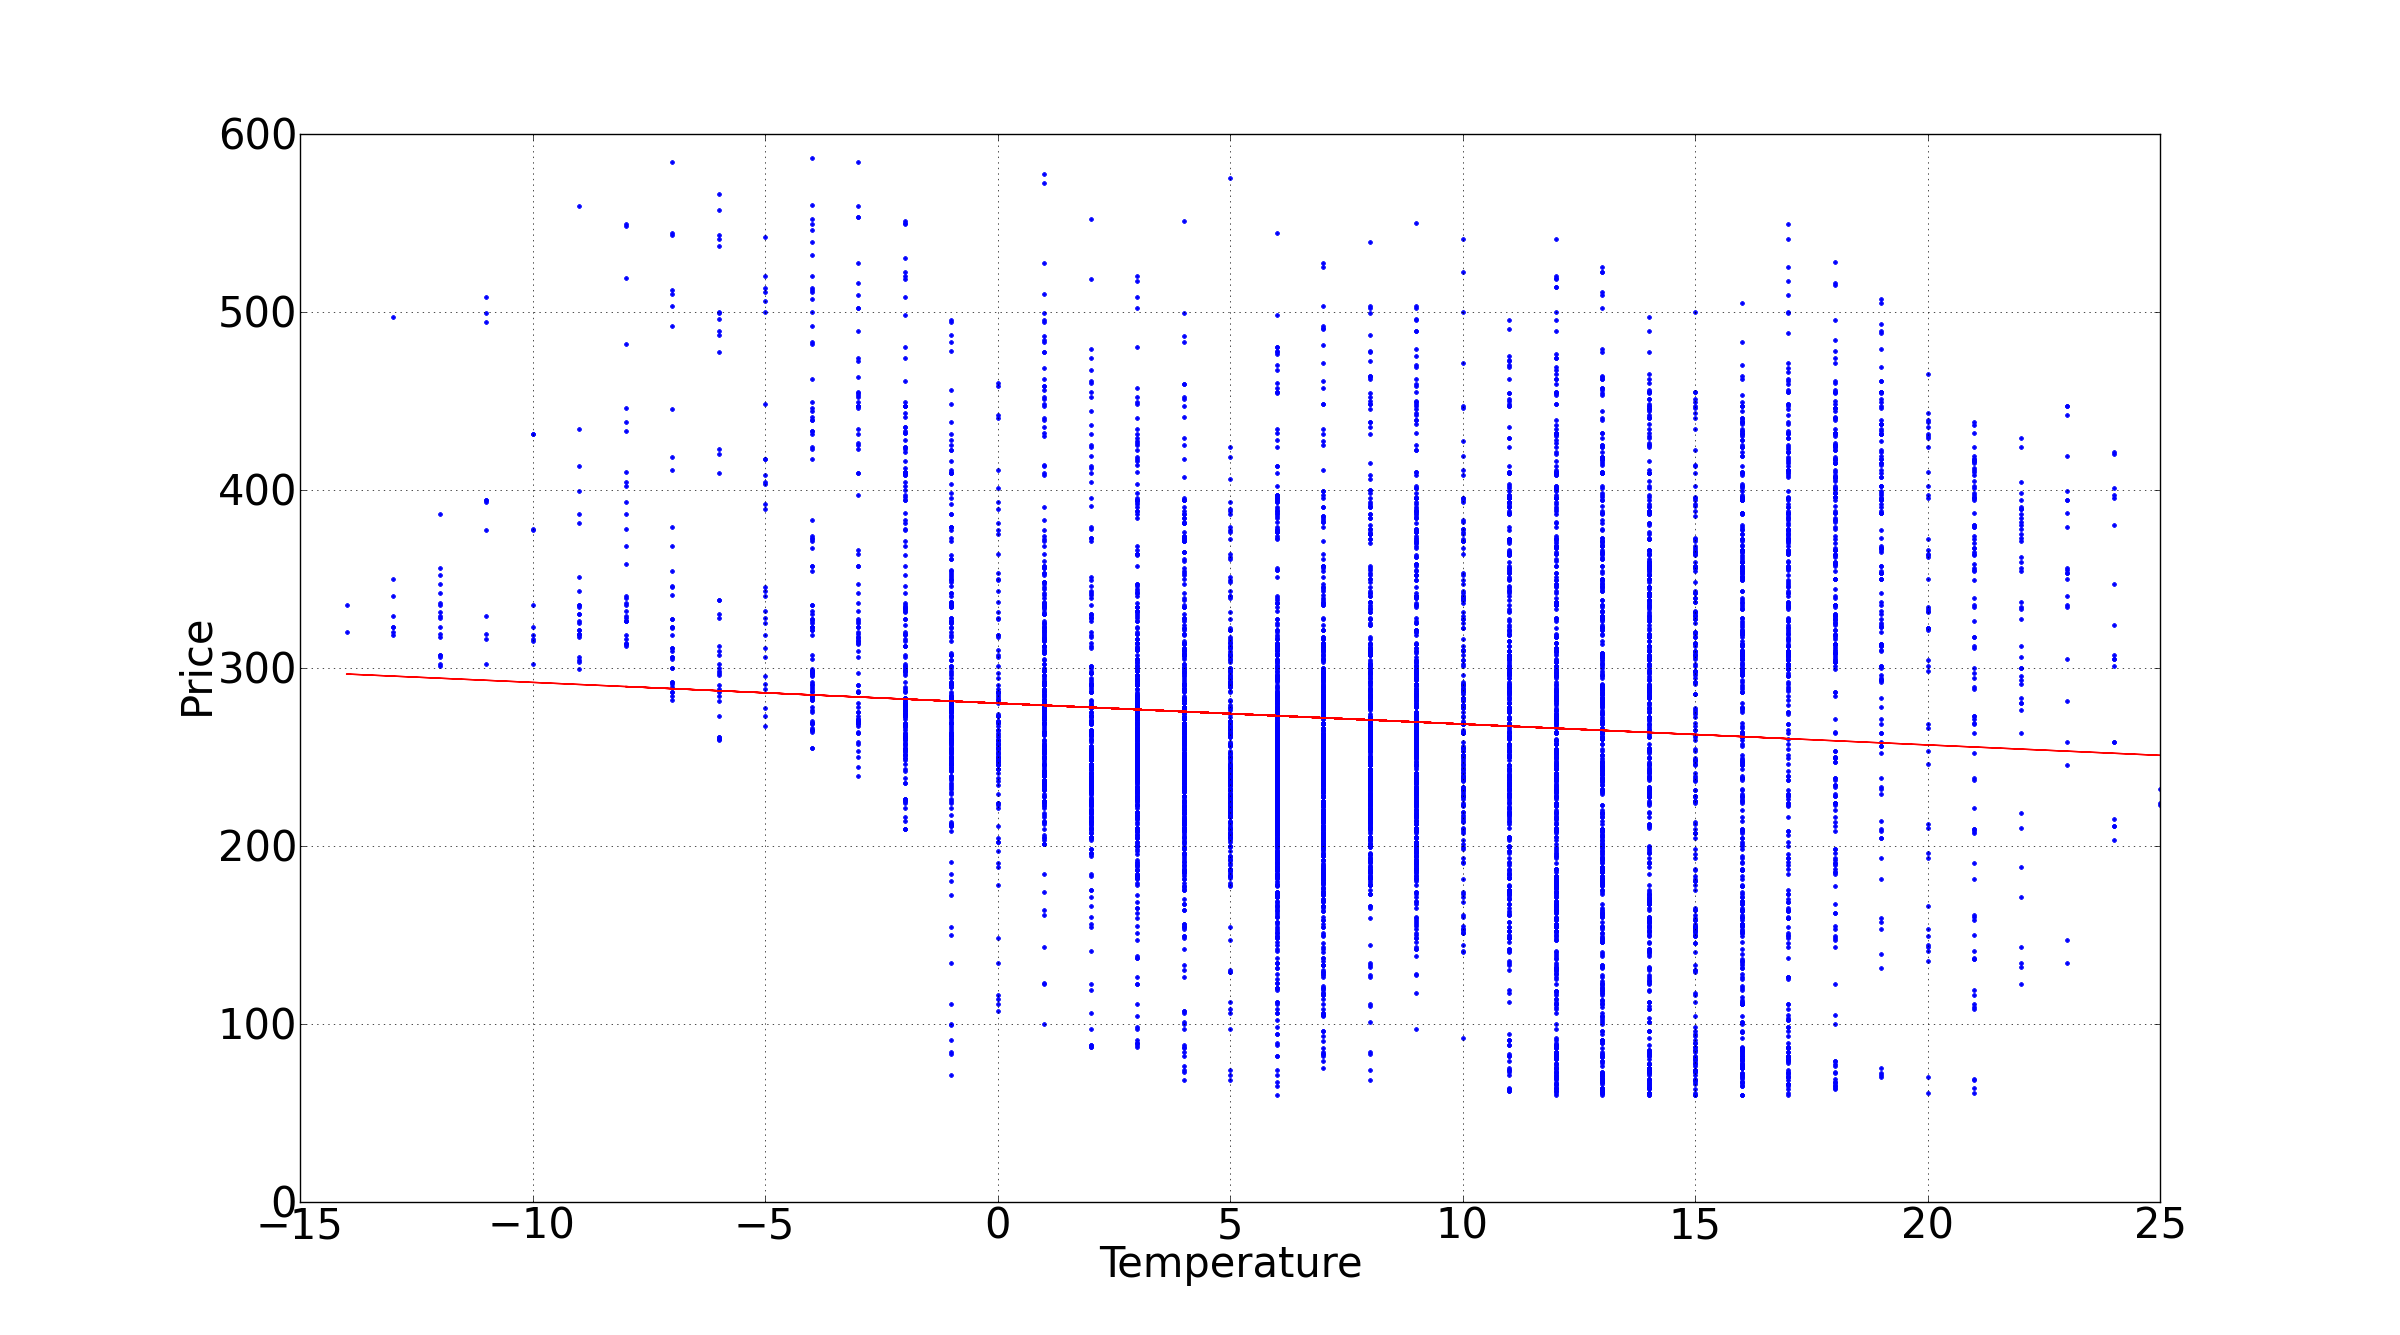
\includegraphics[width=0.99\textwidth]{billeder/energy_price_plots/price_temp.png}
\caption{Price and temperature plot.}
\label{fig:price_temp}
\end{figure}

In Figure~\ref{fig:price_temp} and Table~\ref{table:pearsonsPriceVariables} we see that there is nearly no correlation (coefficient is -0,18) between temperature and the price. This indicates that we probably cannot use the temperature as a direct influence on the price. The temperature variable says something about heating degree days and cooling degree days mentioned in \cite{19}. These days indicate when the need for electrical heating or cooling is present thus influencing the electricity price. This influence is discussed later in this analysis.

\begin{figure}[H]
\centering
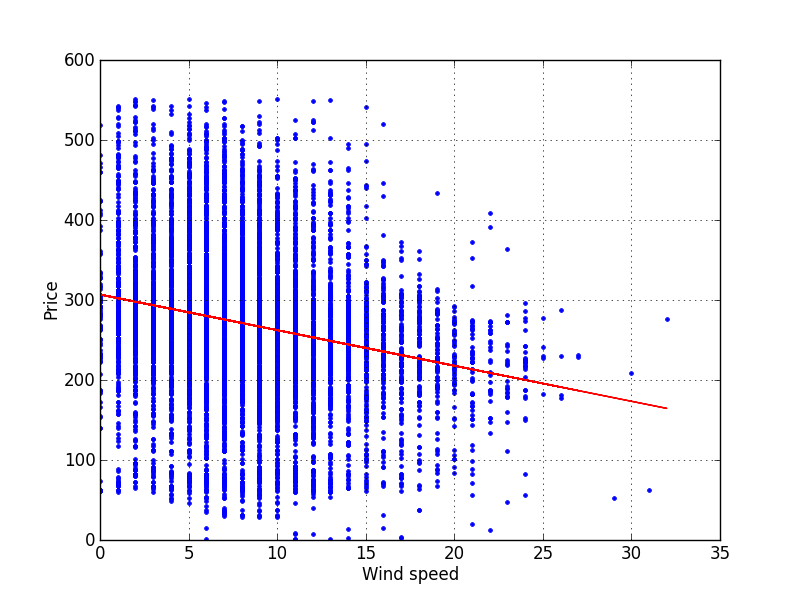
\includegraphics[width=0.99\textwidth]{billeder/energy_price_plots/price_wind.png}
\caption{Price and wind speed plot.}
\label{fig:price_wind}
\end{figure}

In Figure ~\ref{fig:price_wind} we see how the wind impacts the price. If the wind speed increases the energy price decreases. This agrees with paper \cite{dayAheadImpactOfWindPowerForecasts} where they show that the wind influences the wind power production. The share of green energy produced from wind mills are approximately 25\% as off 2008\cite{windPowerDanishLiberalized} so we expect to see that the wind will have an impact on the price. When the production is high and the demand is moderate --- the price will drop because of overproduction and because we cannot store the energy for later use.

%------------------------------------------------------------------------------------------------------------------------------
\subsection{Seasonality}\label{sec:seasonality}
The price is influenced greatly by the seasonality. Seasonality covers the time of year but also the time-of-day and the day-of-the-week in this section. Seasonality plays a significant role in price prediction because the demand is affected by the behaviour of people.

\begin{figure}[H]
\centering
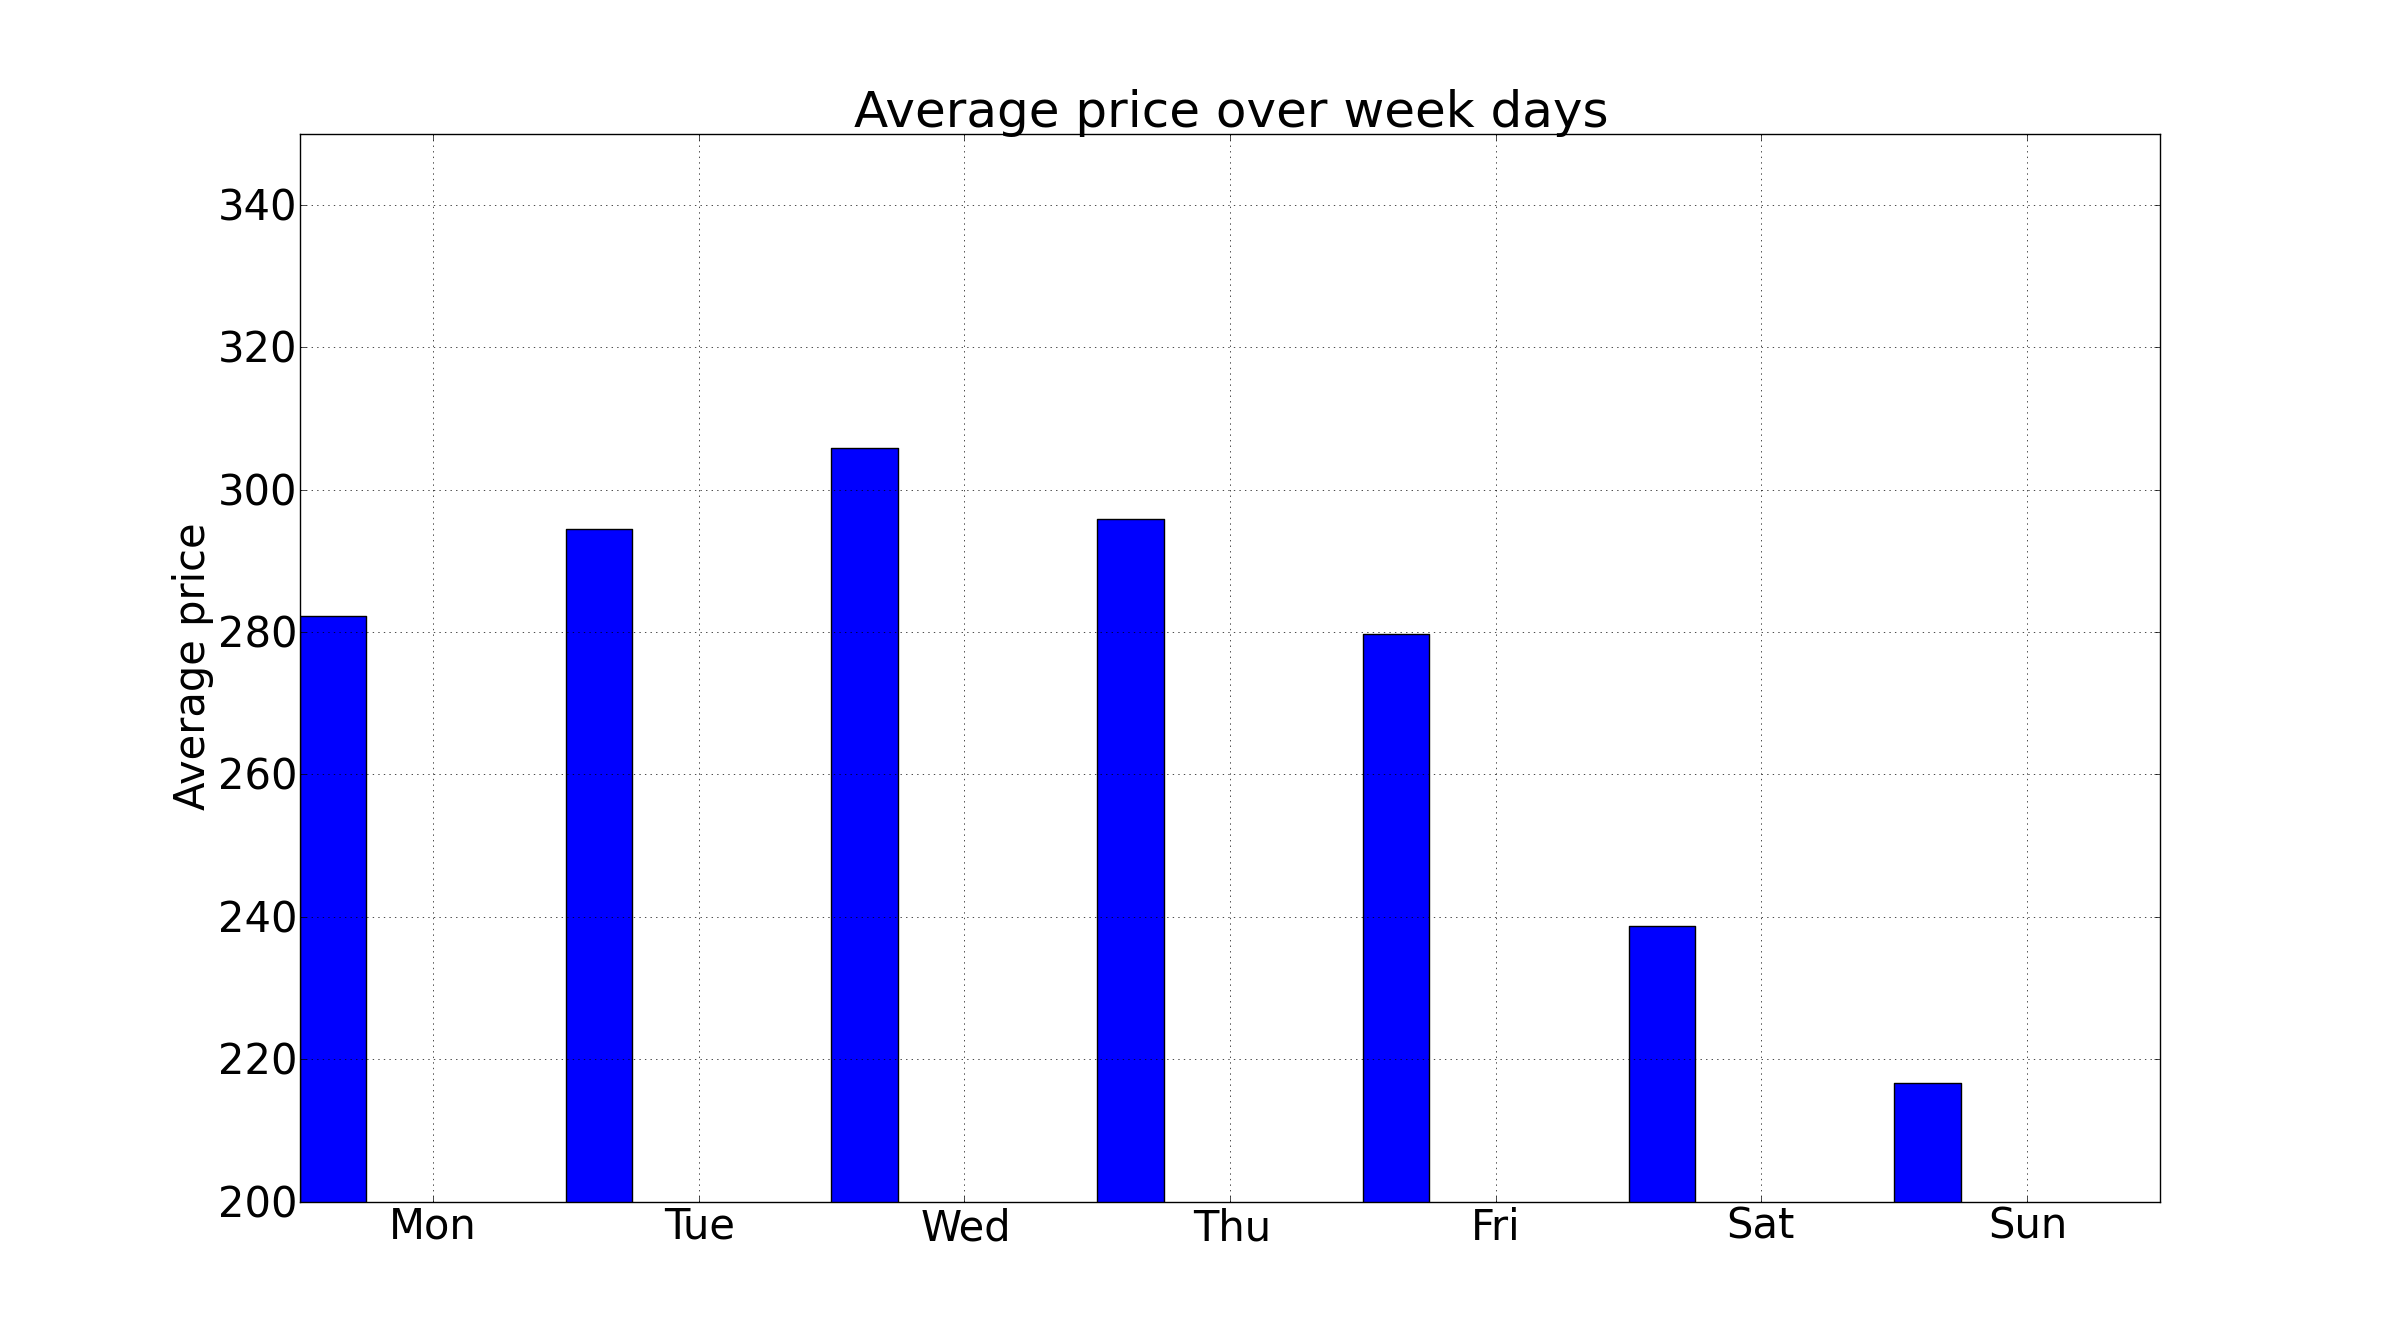
\includegraphics[width=0.99\textwidth ]{billeder/energy_price_plots/Average_price_over_weekdays.png}
\caption{Daily price dispersion}
\label{fig:price_over_weekdays}
\end{figure}

Figure ~\ref{fig:price_over_weekdays} shows us how the trend of the price varies over the different days in a week. The most noticeable here is how the price is decreasing in the weekend (Saturday and Sunday) and are somewhat steady for the weekdays. We are looking at two options for our neural network. The graph shows us a difference between highest (Wednesday) and lowest (Sunday) of 80 which is pretty much when the price fluctuates between 632 and 61 (with 1\% top and bottom trim see section ~\ref{sec:Trimming}).

\begin{figure}[H]
\centering
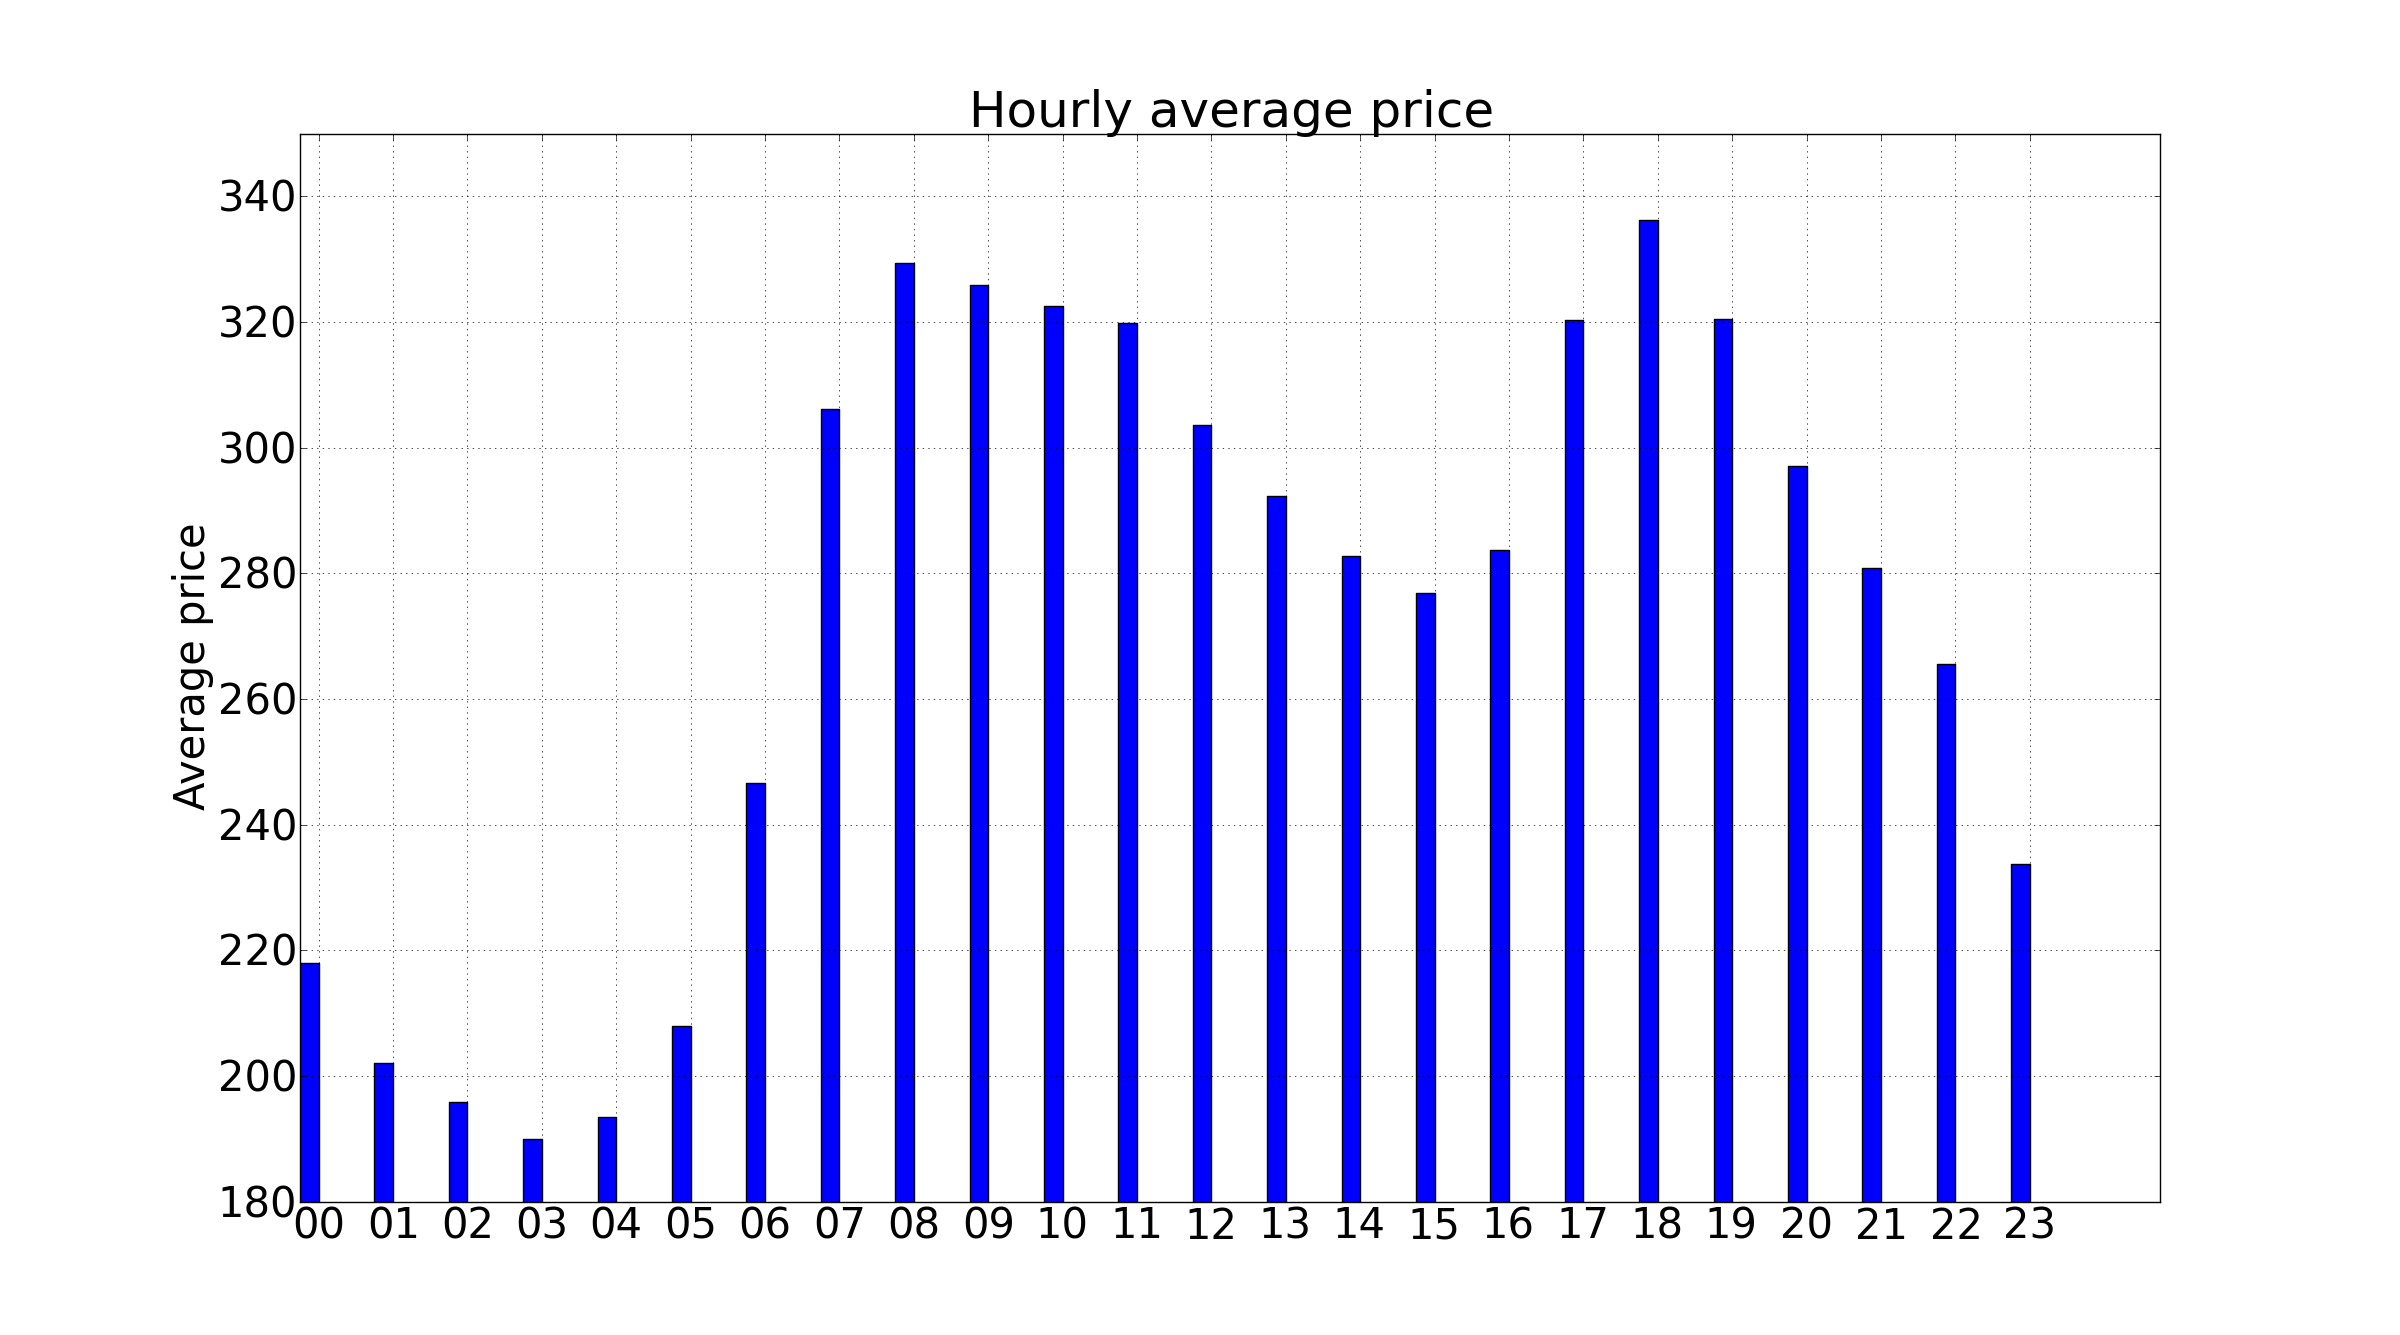
\includegraphics[width=0.99\textwidth ]{billeder/energy_price_plots/price_per_hour.png}
\caption{Hourly price dispersion}
\label{fig:price_per_hour}
\end{figure}

In Figure~\ref{fig:price_per_hour} we see the average price per hour over a whole day. We see a trend where the price is highest from 08 to 10 and again from 17 to 19. This is because the electricity follows the same pattern as people e.g. 17 to 19 is when most people prepares dinners and thus the need for electricity price rises. The price fluctuates between 335 and 190 that gives us a difference of 145. This is a pretty significant difference between highest and lowest and will help us point the prediction in the right direction.

\begin{figure}[H]
\centering
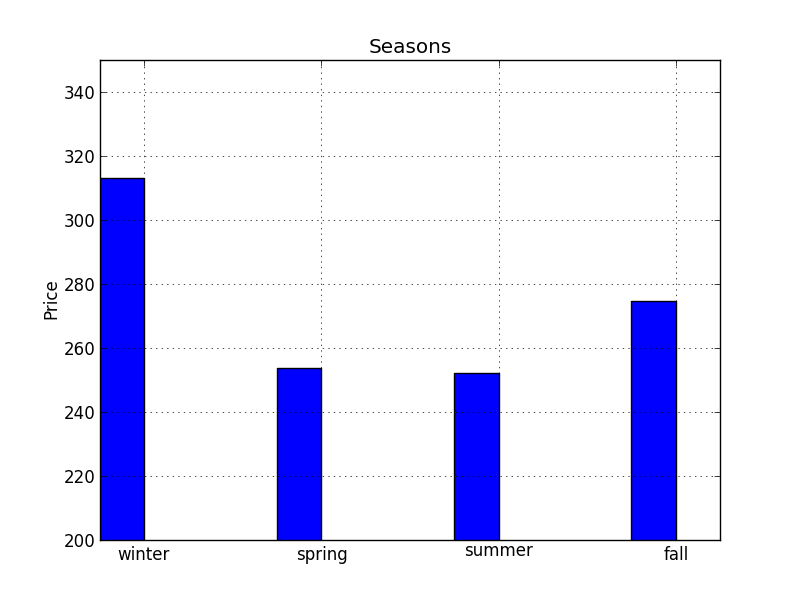
\includegraphics[width=0.99\textwidth ]{billeder/energy_price_plots/seasons.png}
\caption{Seasonal price dispersion}
\label{fig:seasons}
\end{figure}

The sesonality is also reflected in what time of year it is. In the winter time the electrical heating and need for electric light plays a significant role on how much electricity is consumed and thus the price goes up \cite{crowley2005weather}. This is shown in figure ~\ref{fig:seasons} where it clearly shows the average price is higher in winter and fall than in summer and spring.

\begin{figure}[H]
\centering
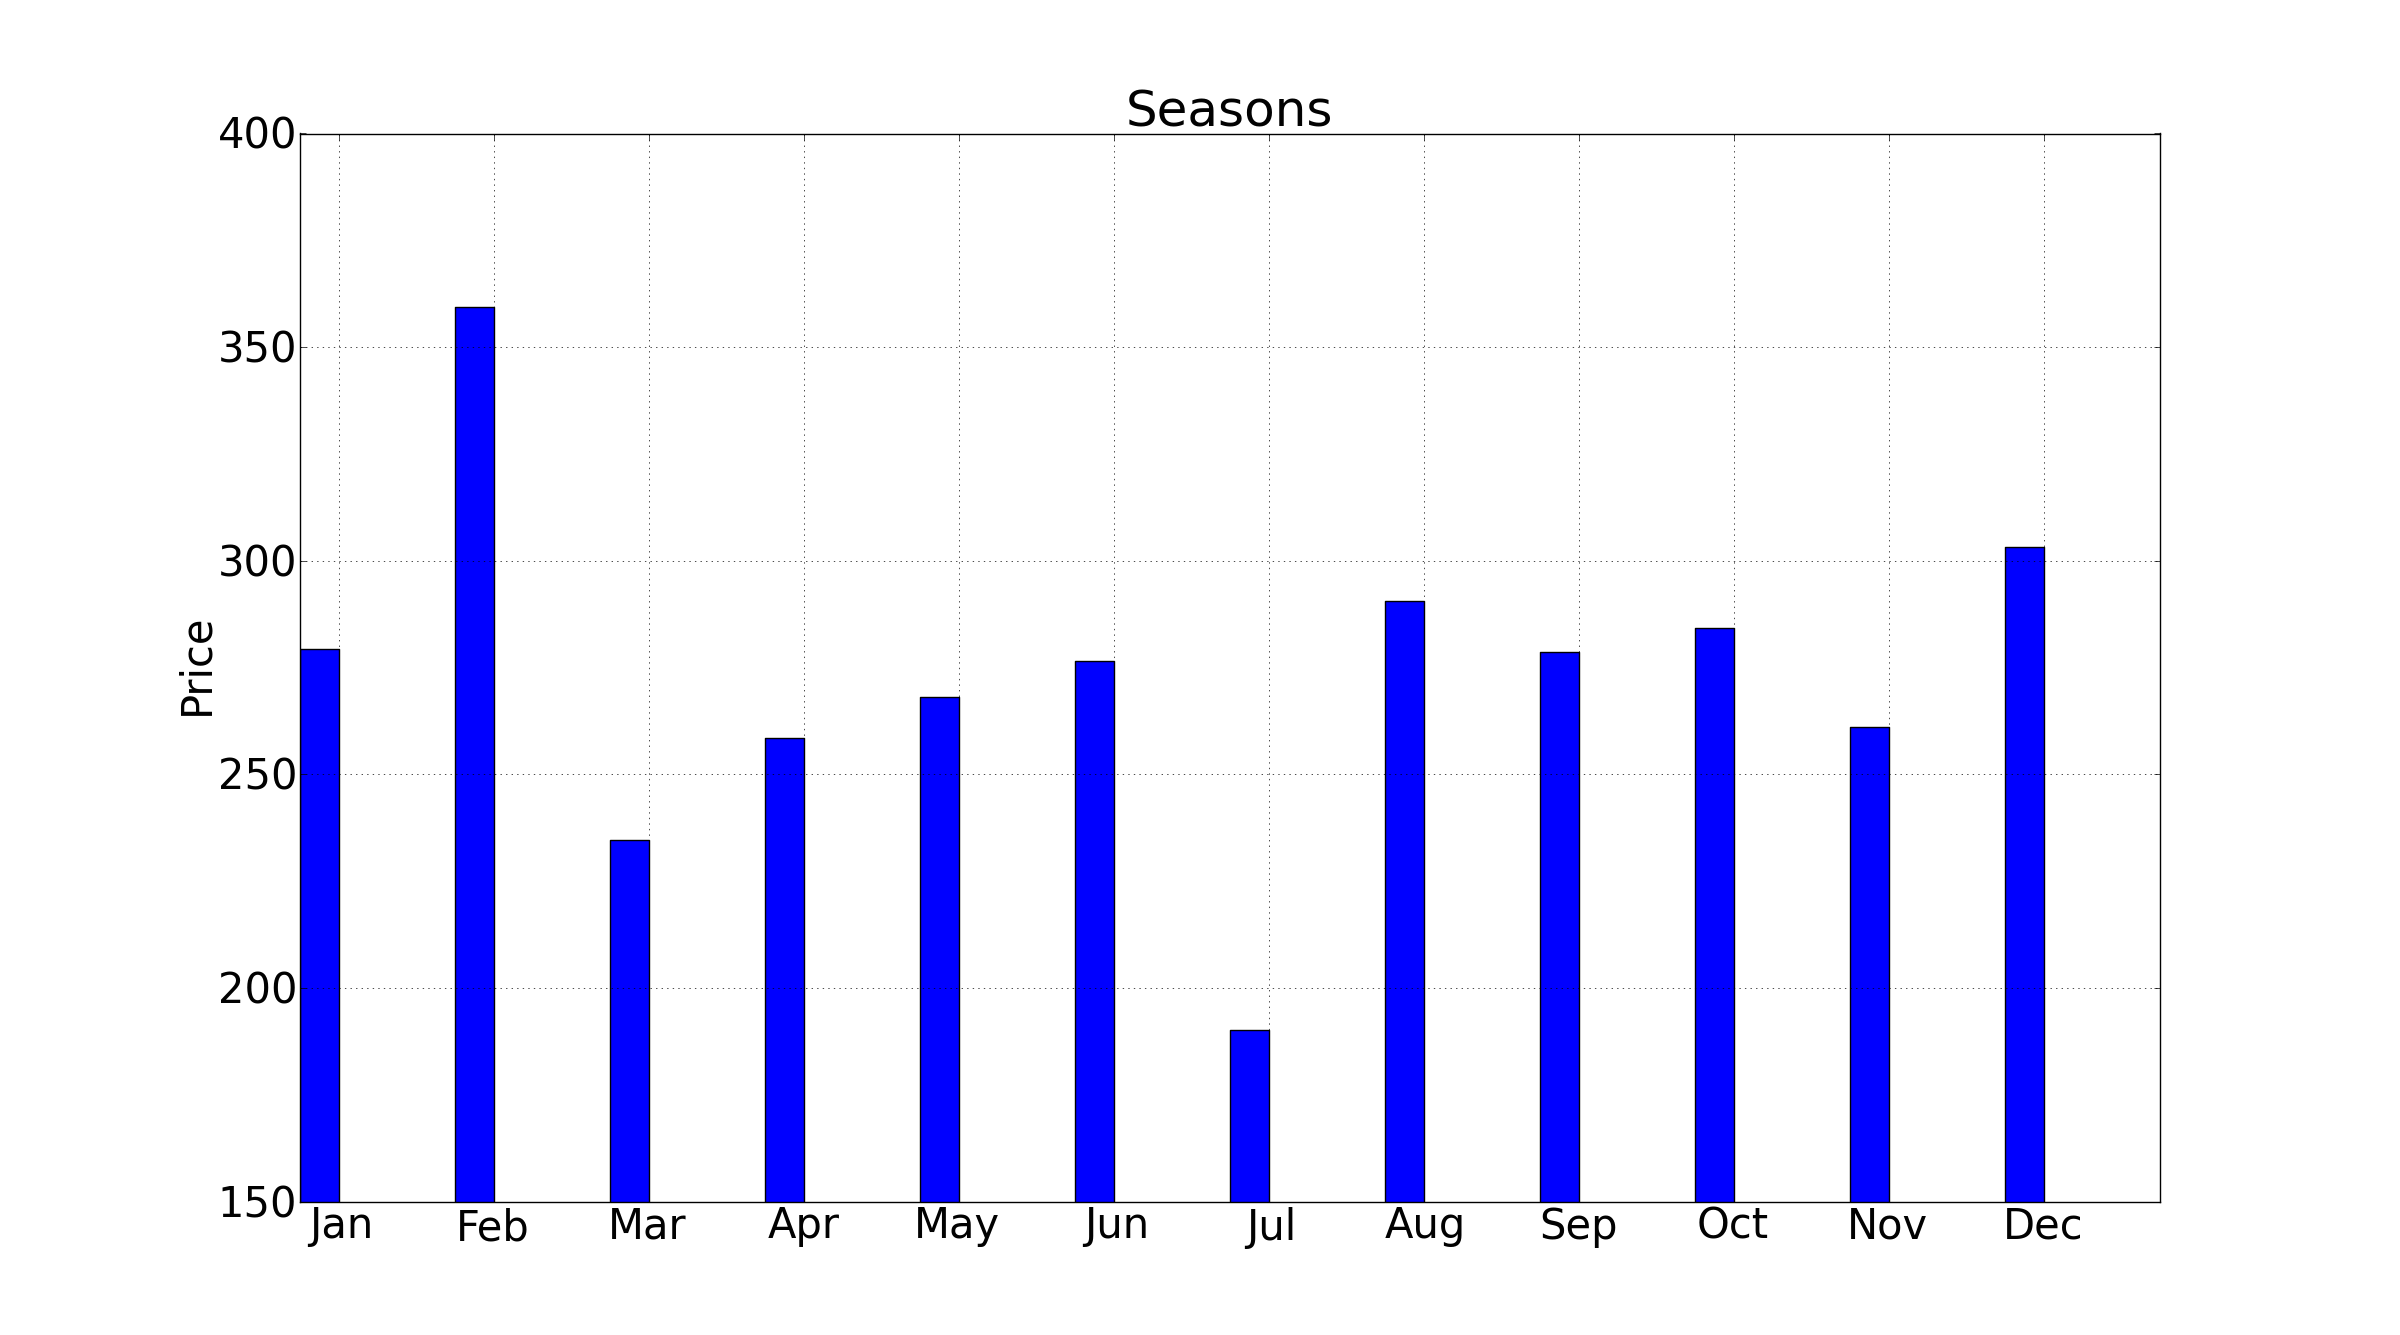
\includegraphics[width=0.99\textwidth ]{billeder/energy_price_plots/averageMonthlyPrice.png}
\caption{Monthly price dispersion}
\label{fig:monthlyAveragePrice}
\end{figure}

To get a more fine grained representation of the seasonal influences on the price; we have created a monthly distribution of the price. The Figure~\ref{fig:monthlyAveragePrice} shows that the highest average price is 360 (February) and lowest 190 (July). This is a significant price jump and shows the same trend as for the seasonal Figure~\ref{fig:seasons} but here we see the effects of the holidays in July; where the price is significantly lower than the rest of the year.

%------------------------------------------------------------------------------------------------------------------------------
\subsection{Volatility and High-Frequency}
\label{sec:volatility}
The electricity prices are very volatile and changes on an hourly basis. The electricity price is one of the most volatile entities in the commodity markets \cite{pjmForecast} if not the most volatile as they state in \cite{yamin2004adaptive}. The spikes are often reflected by the same input variables resulting in completely different results. The price has a very high frequency of spike prices. A spike price is a price that elevates very quickly and drops in a matter of a few hours. These conditions can be tricky to handle and we will now address some of the problems in handling volatility and spike prices.

In \cite{singhal2011electricity} they describe the factors that influence the price and causes them to be highly volatile:
\begin{itemize}
	\item Volatility in fuel price
 	\item Load uncertainty
 	\item Fluctuations in hydroelectricity production
 	\item Generation uncertainty (outages)
 	\item Transmission congestion
 	\item Behavior of market participant (based on anticipated price)
 	\item Market manipulation (market power, counterparty risk)
\end{itemize}
All of these factors influence the price and makes it highly volatile. These factors are very hard to account for and are not included in our analysis but has to be kept in mind when trying to predict the prices. 

Some of these factors will automatically be accounted for when we do the data analysis. They describe in \cite{yamin2004adaptive} that the behavior of the market participants (or the bidding strategies as they call it) are already a part of the training dataset thus already accounted for when we do the analysis of the data.

Spikes are hard to predict and often impossible because of the limited occurrence of these (under 2\% in our dataset) and because they are so much higher than the rest of the max prices. Spikes can add an error factor to the dataset thus making it harder to predict the rest of the datasets values because the ANN will make adjustments for these high values. Trimming can be used to reduce the number of irregular spikes in the datasets and have been used in \cite{singhal2011electricity} where they remove the electricity prices above \$70 and also in \cite{yamin2004adaptive} where they trim the dataset if the price is above \$50. The trimming of course only makes sense to use if it actually improves the predictions. It must be included in experiments to see if it has any improvement.

\begin{figure}[H]
\centering
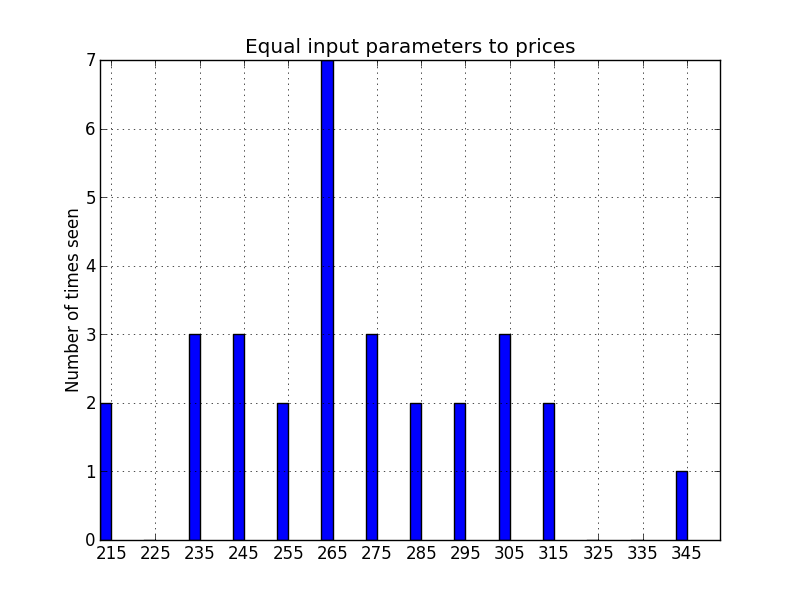
\includegraphics[width=0.99\textwidth ]{billeder/energy_price_plots/same_hour_distribution.png}
\caption{Price ditribution over equal hours}
\label{fig:same_hour_distribution}
\end{figure}

In earlier figures we have shown how the inputs influence the electricity price and given some reasons to why this influences the price. In figure~\ref{fig:same_hour_distribution} we have chosen similar hours across all days of a year and we show how different the price can be for similar inputs. The similar days have been chosen from the 'core' inputs (wind speed, temperature and demand) and the margins seen in table~\ref{table:similarHoursLimits} reflects the upper and lower bound of the inputs. The margins are calculated from a randomly chosen day and the interval is 10\% up and down. Even though the price is volatile we can see a trend in the graph that shows us that the price most of the time will be about 265.

\begin{table}[H]
\centering  % used for centering table
\begin{tabular}{|c|c|c|c|} % centered columns (3 columns)
	\hline
 & Windspeed & Temperature & Demand \\ [0.5ex] % inserts table 
%heading
\hline                  % inserts single horizontal line
High margin: & 12.1 & 6.6 & 2510  \\ \hline
Low margin: & 9.9 & 5.4 & 2053 \\  \hline
\end{tabular}
\caption{This is the high and low margins for our similar hours comparison.} % title of Table
\label{table:similarHoursLimits} % is used to refer this table in the text
\end{table}

\begin{figure}[H]
\centering
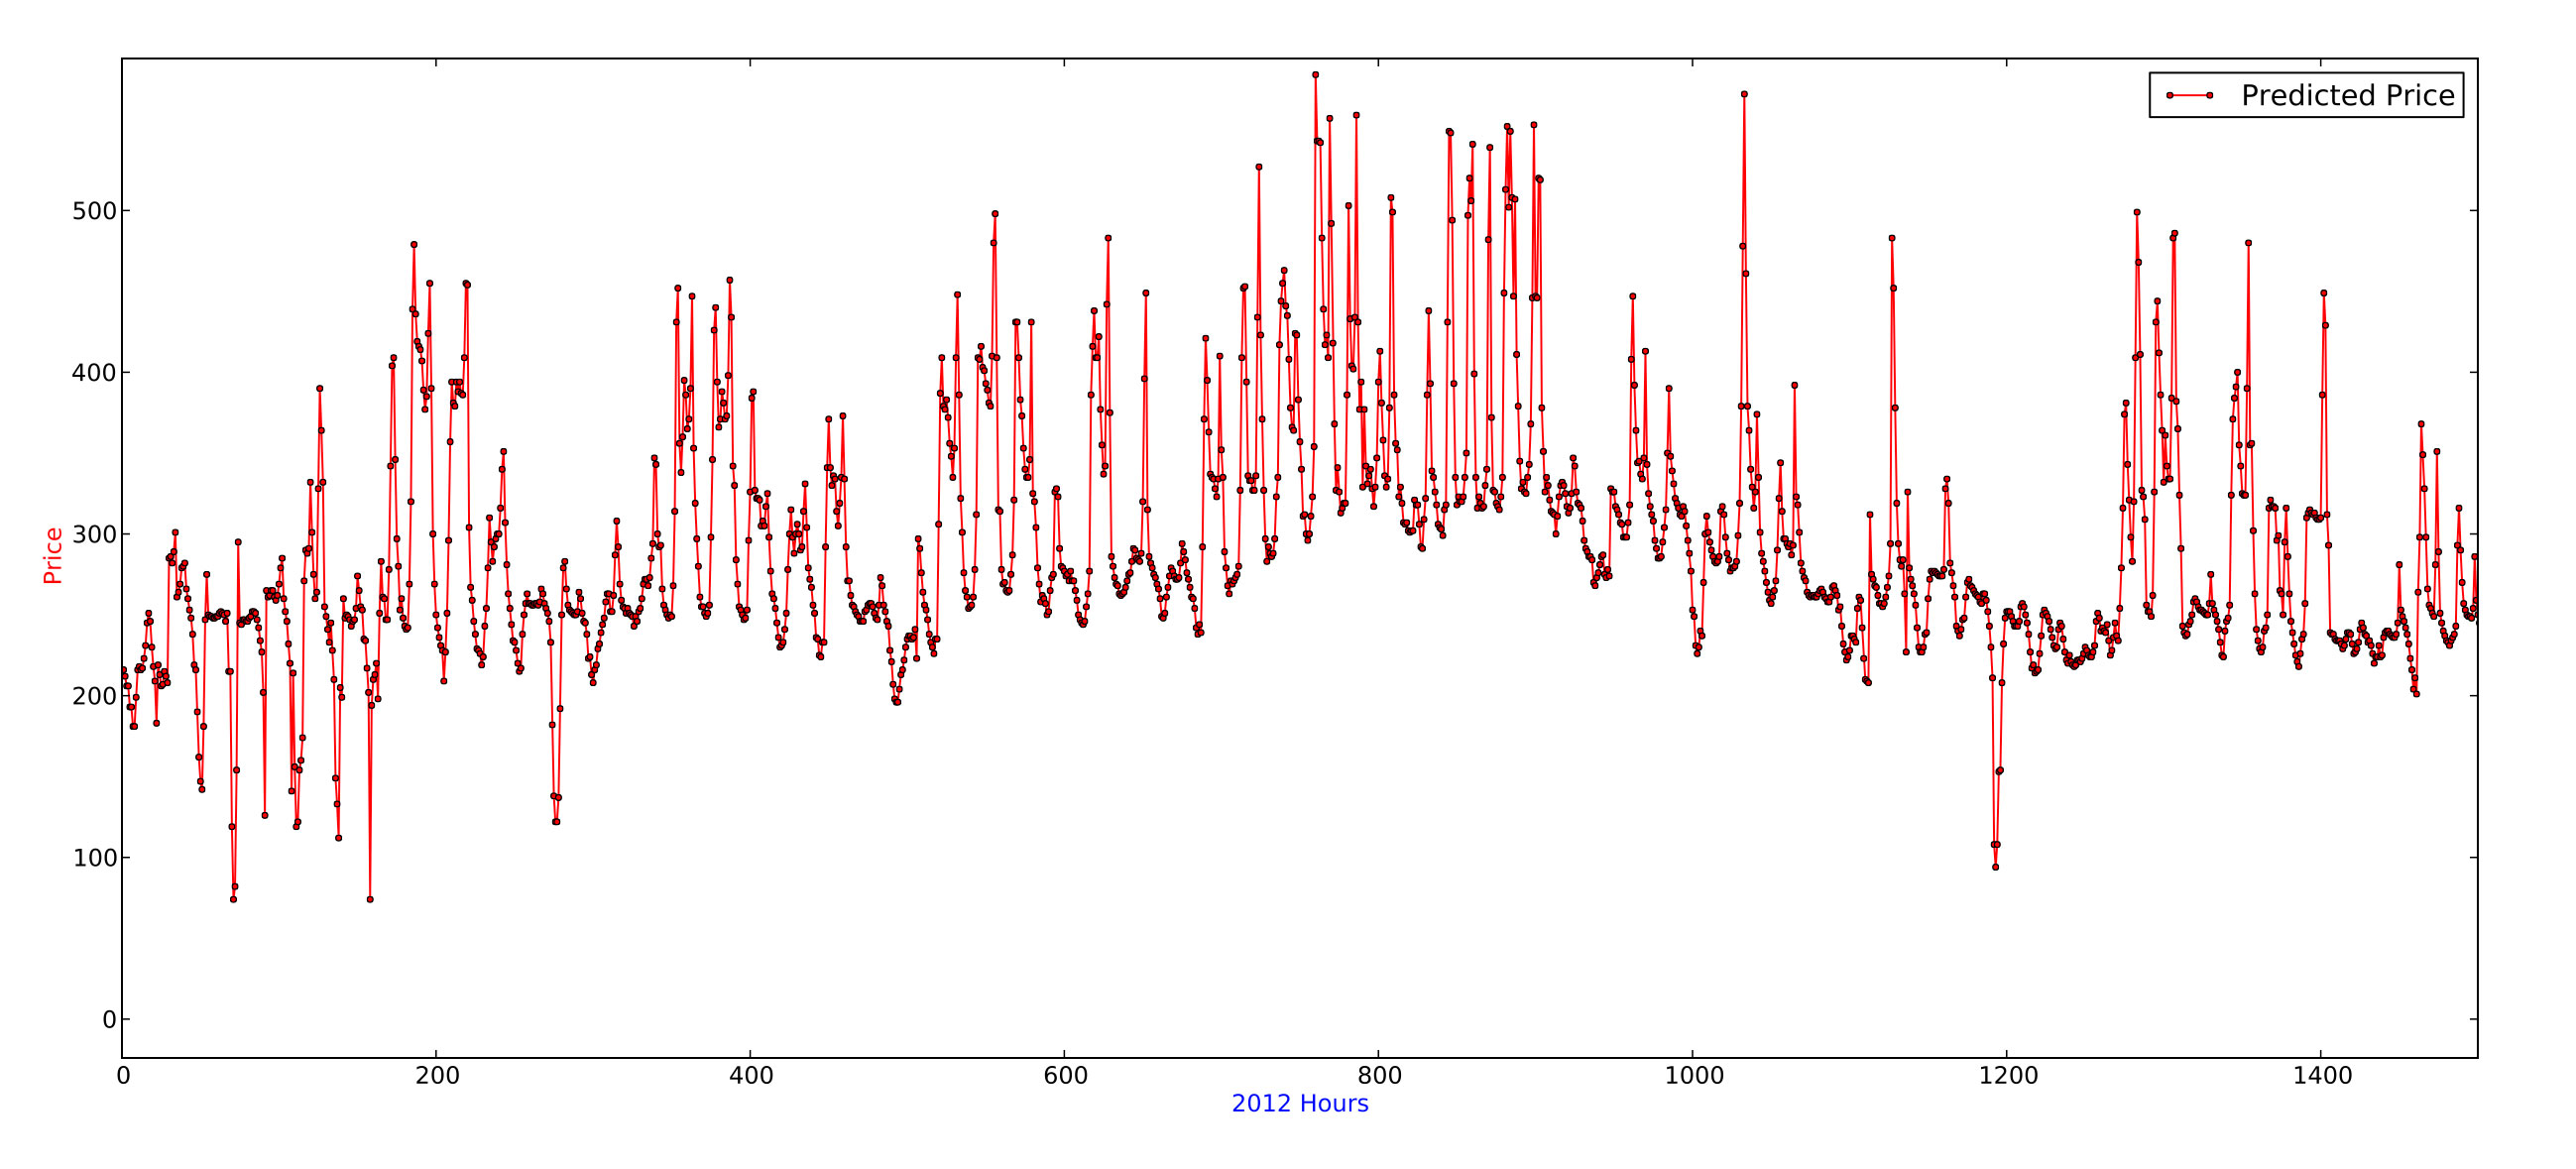
\includegraphics[width=\textwidth ]{billeder/energy_price_plots/plotGraph.jpg}
\caption{A plot graph of the price development over the first 1500 hours in 2012}
\label{fig:plotGraph}
\end{figure}

The volatility of the price is clearly shown in Figure~\ref{fig:same_hour_distribution} where the price on similar hours fluctuates from 215 to 345. To address the volatile nature of the price we need to look at the trends of the known historical price. If we take a look at the price plot in Figure~\ref{fig:plotGraph} it clearly shows how volatile the price actually is. Another thing we can derive from the graph is how the price moves. It does not just jump from top to bottom of the interval but it takes (in most cases) intermediary steps to get there. This tendency can be used alongside the last known price to give the neural network a direction to follow and an approximate price as a point of origin. For more details on this see section~\ref{sec:usingStatisticalInput}.

In the same manner we can address the high-frequency spike prices that occurs in the time series. We have to identify a tendency in the historical data and use this to make the predictions follow the steep spikes in the dataset.

%------------------------------------------------------------------------------------------------------------------------------
\subsection{Demand}
Demand is directly connected to the energy prices (which comes as no suprise) since every market is driven by demand \cite{singhal2011electricity}. Since demand needs to be predicted we chose to include from \fnurl{Nord Pool Spot}{http://www.nordpoolspot.com/} since it is out of scope for this thesis to predict it. We can though attempt to compute the demand in our Artificial Neural Network by using the influential factors of demand as inputs, i.e. substitute the demand input with the factors that plays a role in predicting the demand. The last two methods requires us to have an idea of what the input parameters for the prediction of demand is. As mentioned in related work we have seen a function that calculates the demand based on CDD(Cooling degree days), HDD(Heating degree days), ELD(Humidity), V$_w$ (Wind speed), M$_s$ (Sunshine), M$_r$ (Rainfall) \cite{19}.

\begin{figure}[H]
\centering
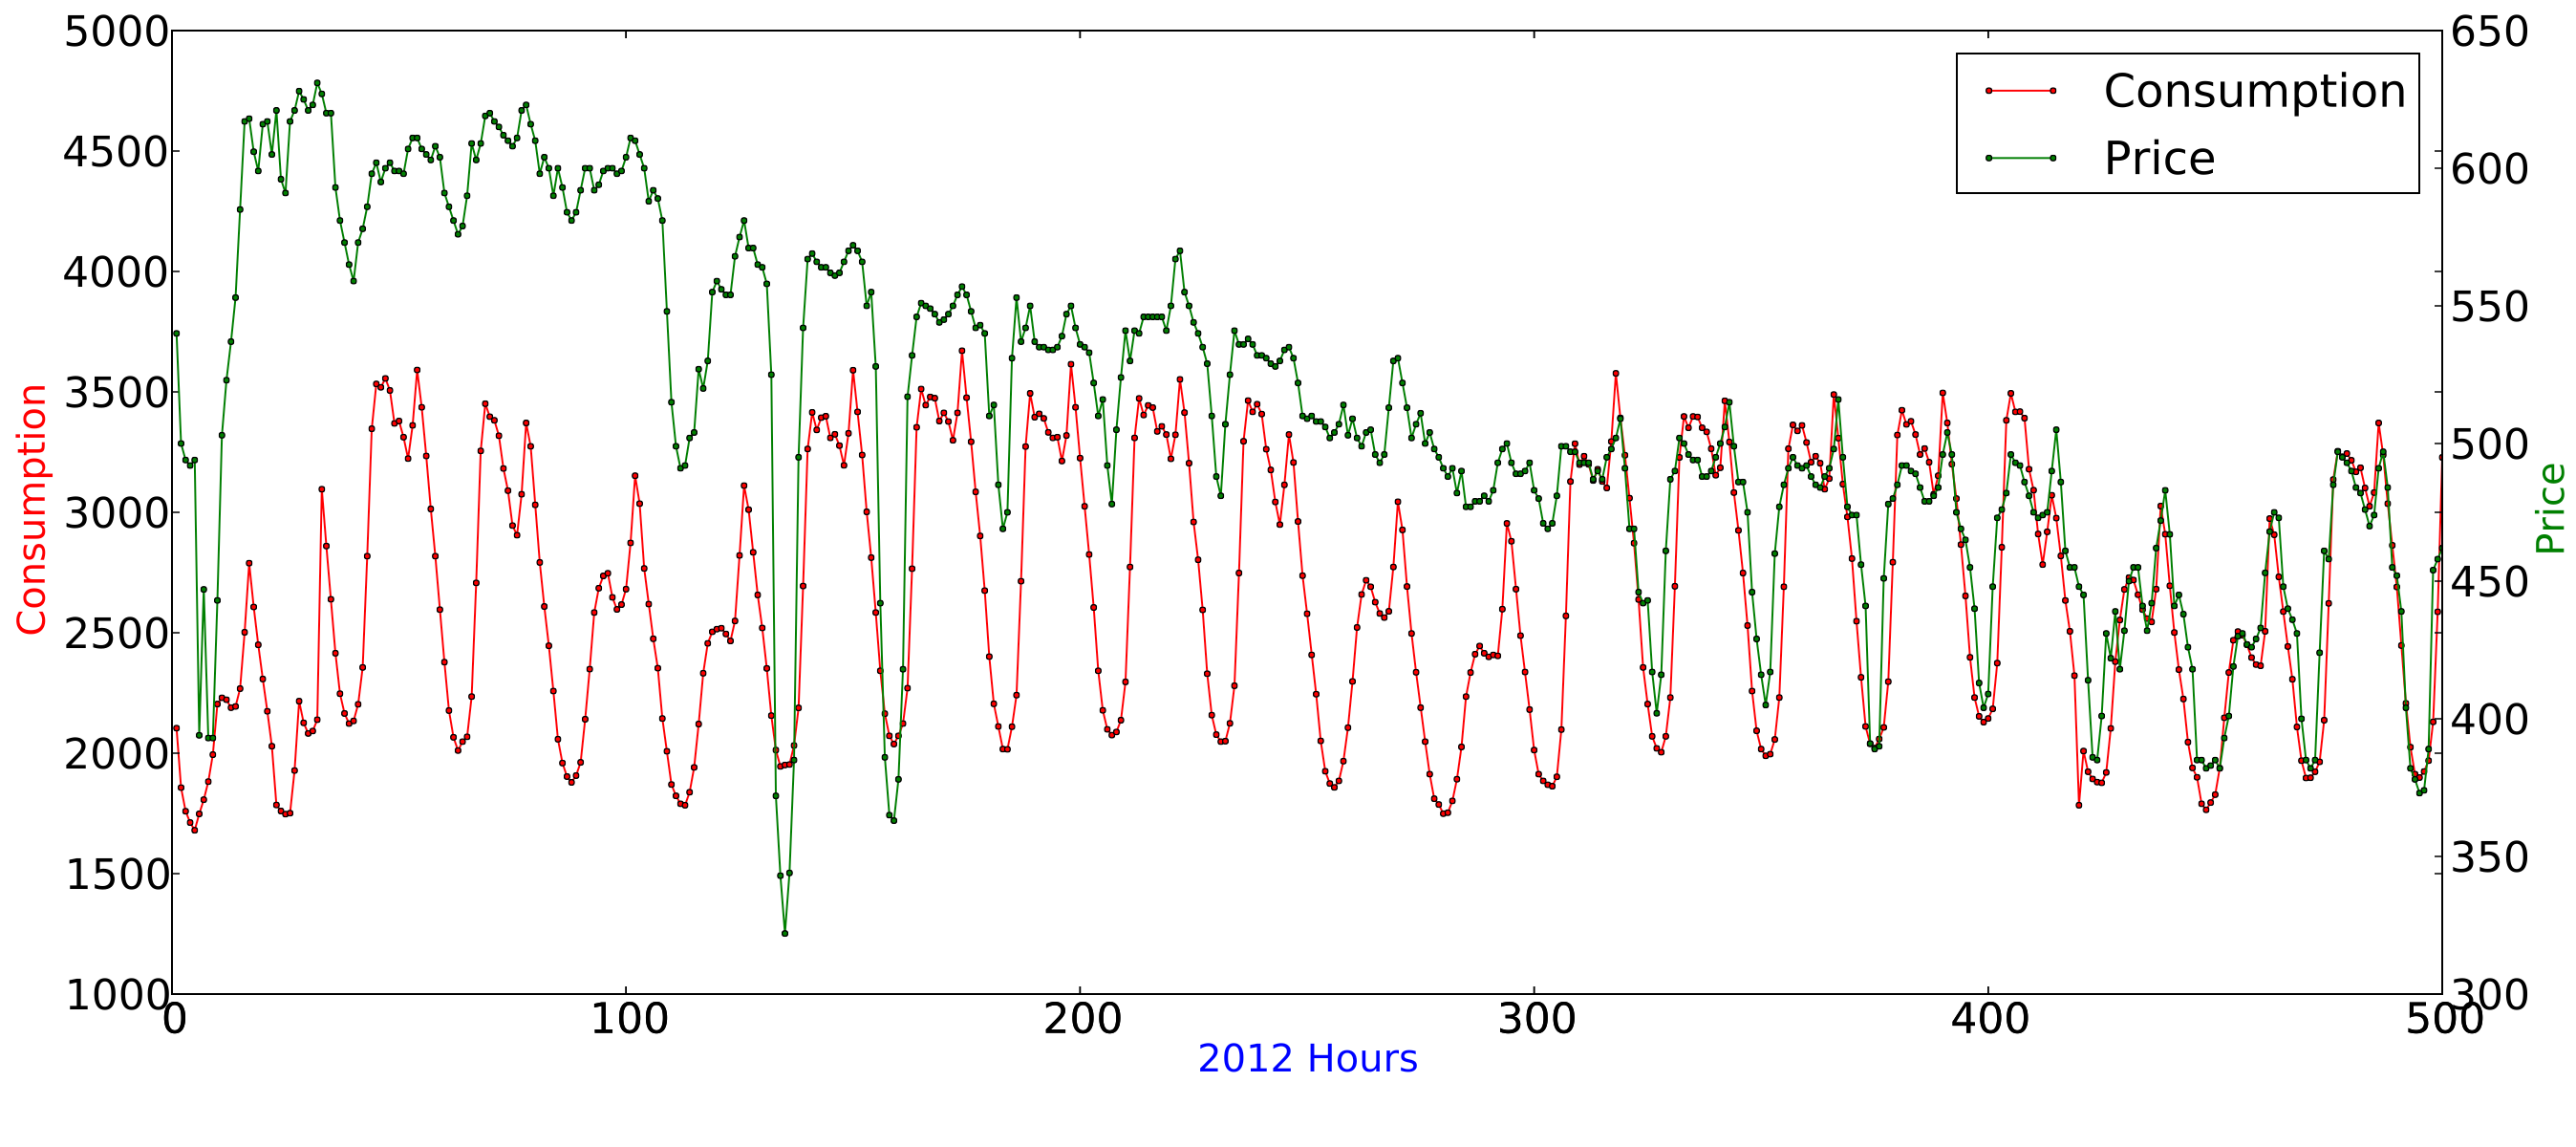
\includegraphics[width=0.99\textwidth ]{billeder/energy_price_plots/price_consump_graph.png}
\caption{Demand and price plot.}
\label{fig:consump_price_graph}
\end{figure}

The price and consumption if mapped out in a graph shows that they follow the same trends see Figure ~\ref{fig:consump_price_graph}. The demand and price does not follow the exact same pattern that also states that there are more factors that influence the price.

\begin{figure}[H]
\centering
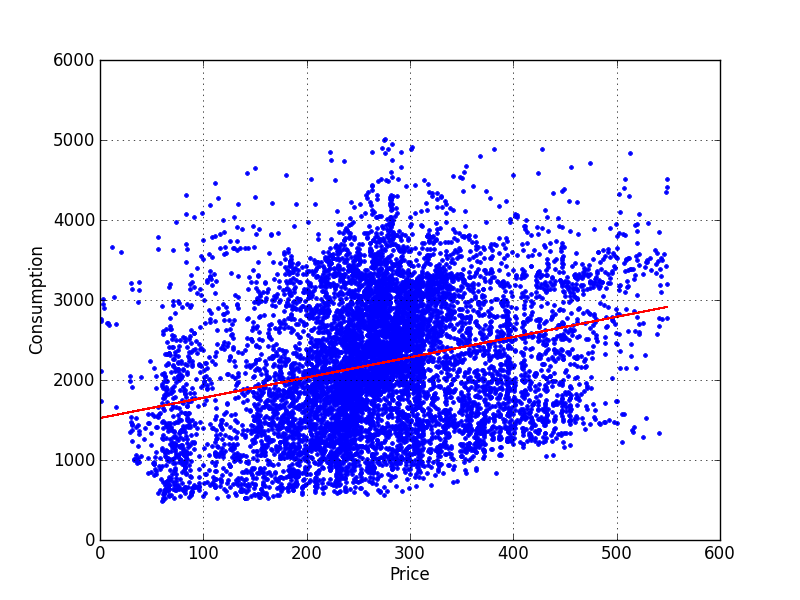
\includegraphics[width=0.99\textwidth ]{billeder/energy_price_plots/consump_price.png}
\caption{Demand and price plot.}
\label{fig:consump_price}
\end{figure}

In Figure ~\ref{fig:consump_price} we see the connection between energy price and the demand. The model shows us that if the demand rises the electricity price rises as well. This is a common tendency in a market where there is not endless supply.

\begin{figure}[H]
\centering
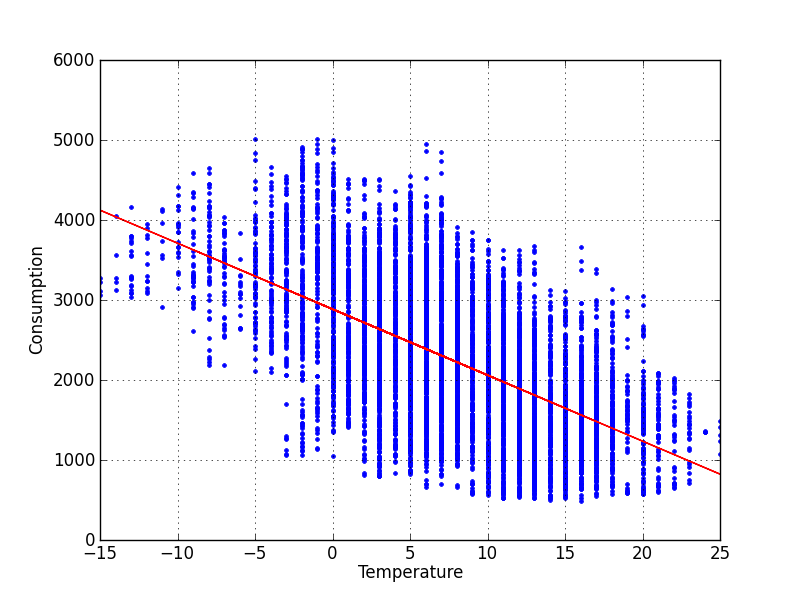
\includegraphics[width=0.99\textwidth ]{billeder/energy_price_plots/consump_temp.png}
\caption{Demand and temperature plot.}
\label{fig:consump_temp}
\end{figure}

In Figure ~\ref{fig:consump_temp} we see the connection between demand and temperature. The temperature itself has an influence when it is very cold or very warm. This connection is expressed as CDD(Cooling degree days) and HDD(Heating degree days). In Figure ~\ref{fig:consump_temp} we see that if temperature decreases the demand will go up. This is because the people of Denmark use a lot of energy on heating their homes and lighting them (HDD) in the winter time. In \cite{19} they also describe CDD which indicates the need for cooling. In Denmark it is limited how high the temperature goes and how often we actually need to cool our homes see table~\ref{table:CDD_HDD}. The table shows that we only have two days that are characterized as cooling degree days. On the other hand we have a lot of heating degree days where we need heating. As they are the majority of the days we will use temperature as a measure for this. CDD and HDD are normally calculated as an index for how much of a need there is for cooling or heating respectively. Here we just present what days are categorized as either and not the index.

\begin{table}[H]
\centering
\begin{tabular}{|c|c|c|} 
	\hline
HDDs seen & CDDs seen & Others \\ [0.5ex]
\hline
315 & 2 & 48 \\  \hline
\end{tabular}
\caption{Number of HDD, CDD and other days seen throughout 2012.} % title of Table
\label{table:CDD_HDD} % is used to refer this table in the text
\end{table}

\begin{figure}[H]
\centering
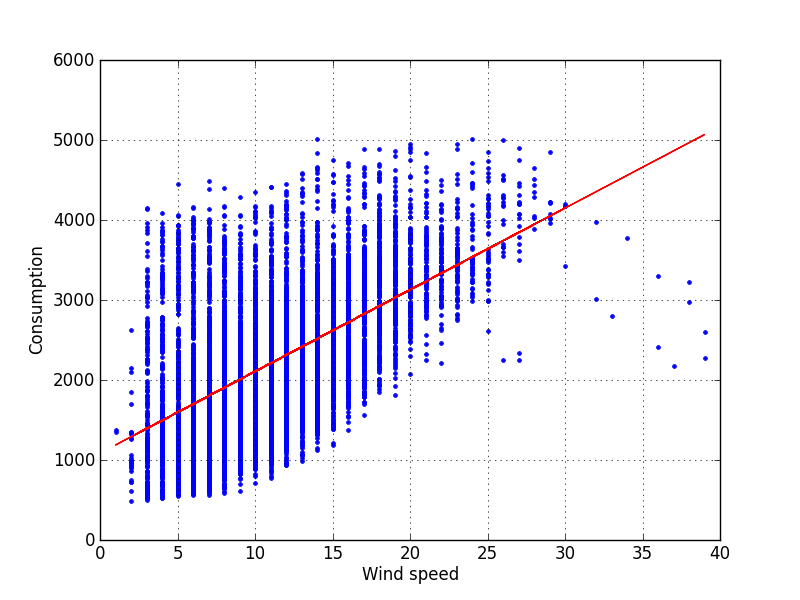
\includegraphics[width=0.99\textwidth ]{billeder/energy_price_plots/consump_wind.png}
\caption{Demand and wind speed plot.}
\label{fig:consump_wind}
\end{figure}

Wind speed plays a role in predicting electrical demand. The wind affects the electrical heating needed in homes across the country. The wind cools down the houses and thus need for heating arises \cite{19}. As seen in Figure ~\ref{fig:consump_wind} and in Table ~\ref{table:pearsonsPriceVariables} there is a pretty good correlation between wind speed and demand. The graph clearly shows us that; when the wind speed increases (from 15 and up) the overall demand increases aswell. This indicates that high wind speeds will have the greatest influence on the demand.


%------------------------------------------------------------------------------------------------------------------------------
\subsection{Conclusion}
The above analysis of the data inputs have shown what parameters are more likely to influence the price than others. The last-known price and the price to predict showed a 0.89 pearsons correlation and a graph that showed a close to linear correlation between the two. The weather conditional factors did not show the most convincing correlations with the price. The wind speed showed the best correlation and are the most likely to show and impact. The seasonality of the data was pictured in graphs and the connection between time of day, day of week, month of year and season of year was pretty obvious. We therefore expect them to have a great impact on the price. The volatility and high frequency section showed us that there might be a need for trimming and a need for graph analysis to make the predictions more accurate. The demand section showed how demand and price followed the same pattern and that they are connected. The Pearsons correlation between the two are not the best but we still expect it to be very important for the accuracy of the predictions.